%%%%%%%%% begin snippet
%% You need to add the package "tabularx".
%% Place the snippet right after \begin{document}

% need tabularx
\documentclass{article}
\usepackage{tabularx}
\usepackage{graphicx}
\usepackage{pdfpages}
\usepackage{listings}
\usepackage{subcaption}
\usepackage{verbatim}

\begin{document}
    \begin{titlepage}
           \begin{center}
                 \begin{huge}
                       %% Update assignment number here
                       \textbf{Assignment 4}
                 \end{huge}
           \end{center}

           \begin{center}
                 \begin{large}
                       Machine Learning 1, SS23
                 \end{large}
           \end{center}

           \begin{center}
                \begin{tabularx}{\textwidth}{|>{\hsize=.33\hsize}X|>{\hsize=.33\hsize}X|>{\hsize=.33\hsize}X|}

                       \hline
                       \multicolumn{3}{|c|}{\textbf{Team Members}} \\
                       \hline
                       Last name & First name & Matriculation Number \\
                       \hline
                       Grassl & Ifeoma & 12011965 \\
                       \hline
                       Royer & Christoph & 12004184 \\
                       \hline

                \end{tabularx}
           \end{center}

    \end{titlepage}

    \section{Maximum Likelihood Estimation}
    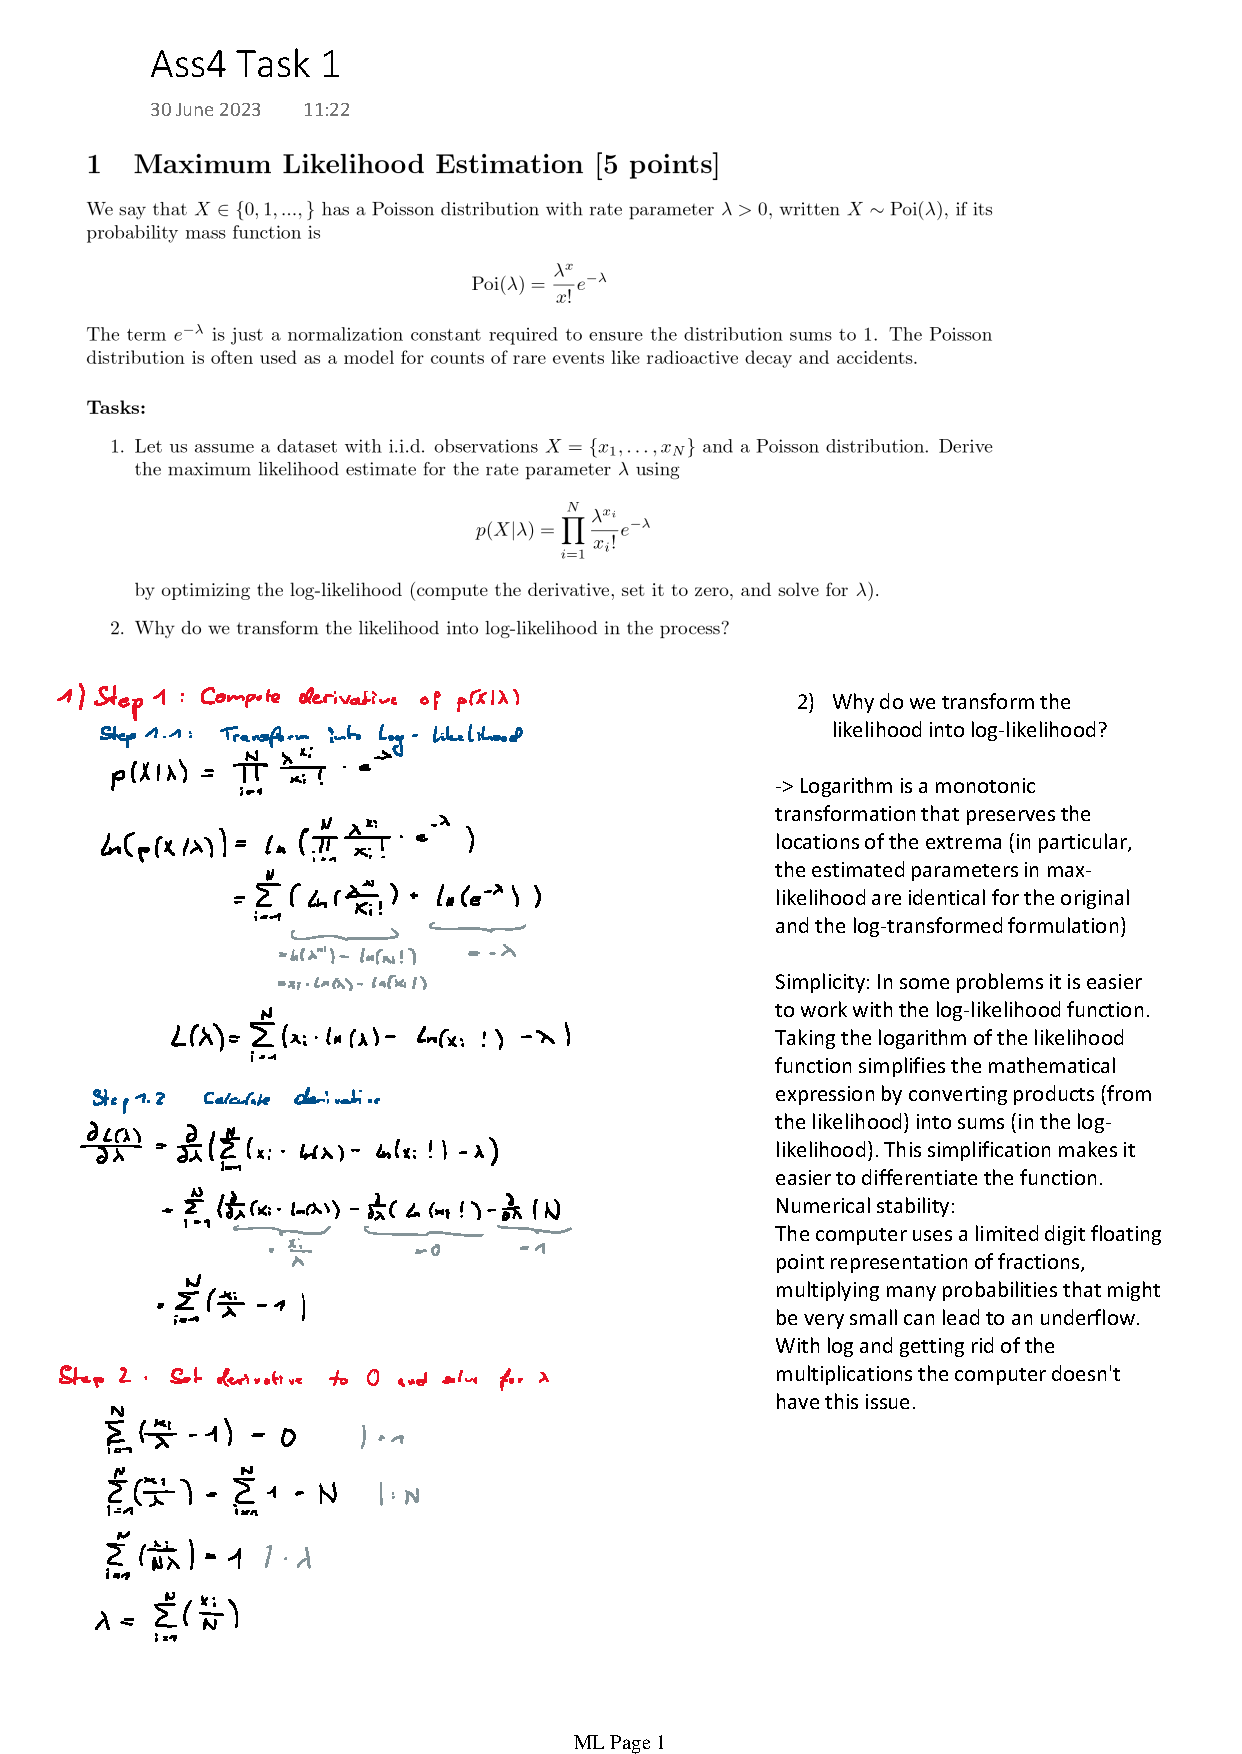
\includepdf[pages={1-1}]{Ass4 Task 1.pdf}

    \section{K-means. Expectation-Maximization Algorithm}
    \subsection{K-means Algorithm}
    \label{subseq:kmeans}
    \textit{See implementation in} \texttt{k\_means.py}

    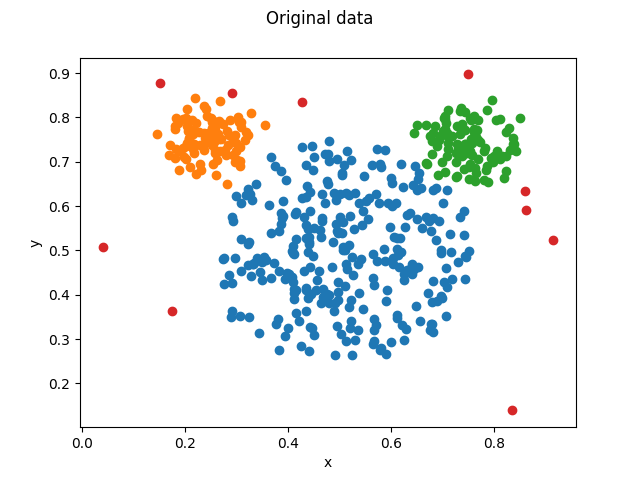
\includegraphics[width=\textwidth/2]{plots/mickey_original} \\
    The original data shows three nearly circular clusters with a few outliers.

    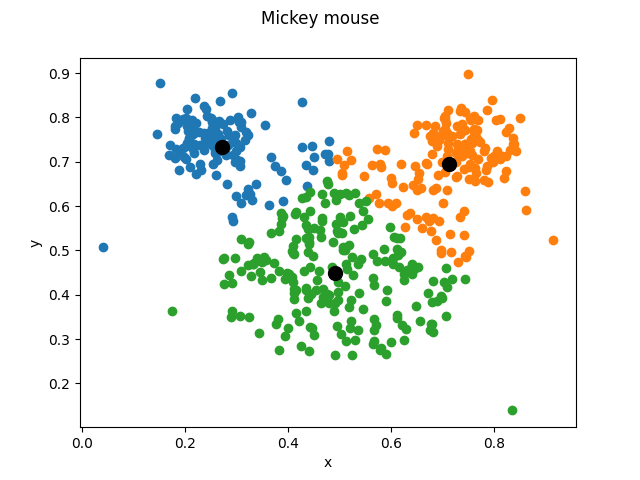
\includegraphics[width=\textwidth / 2]{plots/mickey_k3}
    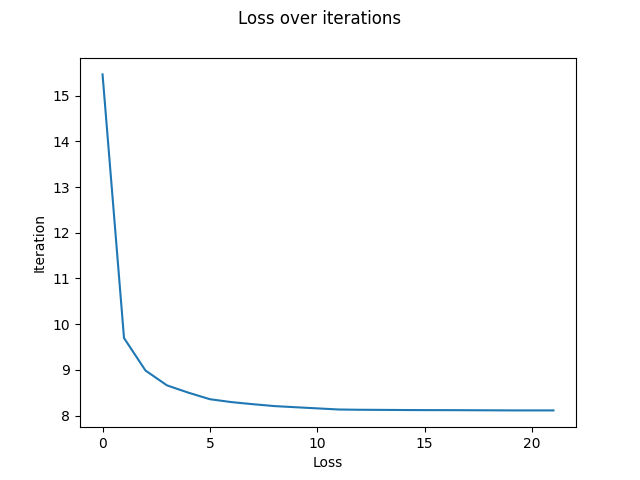
\includegraphics[width=\textwidth / 2]{plots/mickey_k3_loss} \\
    When compared to the original data, a K-means with $K=3$ shows some problems.
    Some of the samples of the main cluster are attributed to the smaller, upper clusters.
    This is because though they would fit better with the big cluster, they are technically nearer to the smaller centroids.

    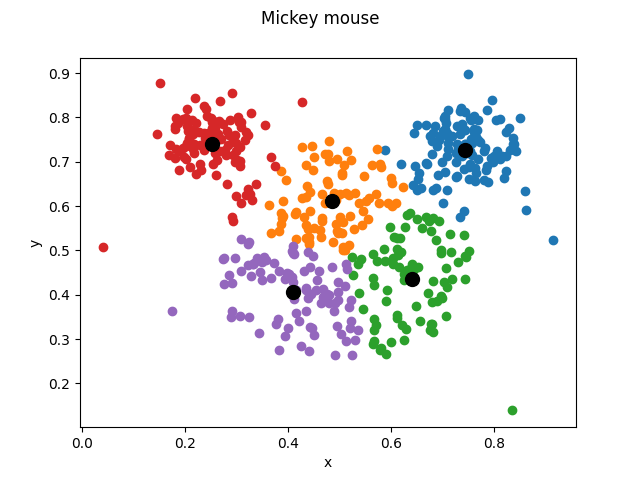
\includegraphics[width=\textwidth / 2]{plots/mickey_k5}
    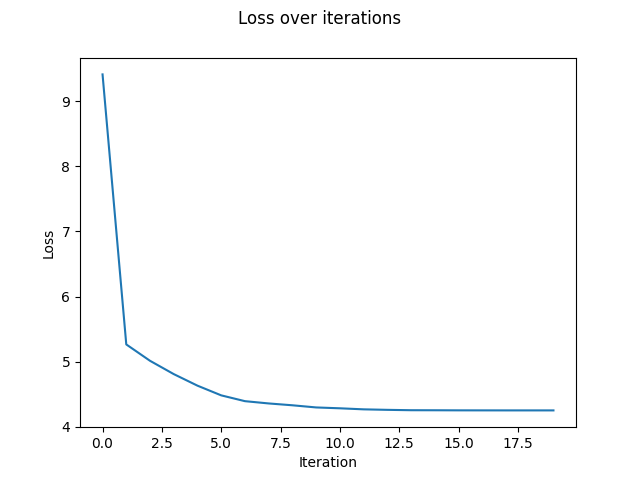
\includegraphics[width=\textwidth / 2]{plots/mickey_k5_loss}
    When setting $K=5$, the problem of the small clusters bleeding into the big one is mostly fixed.
    But now one would manually have to stitch together the three centroids that all take up some of the space in the big cluster.

    \subsection{Expectation-Maximization Algorithm}
    \textit{See implementation in} \texttt{em.py}

    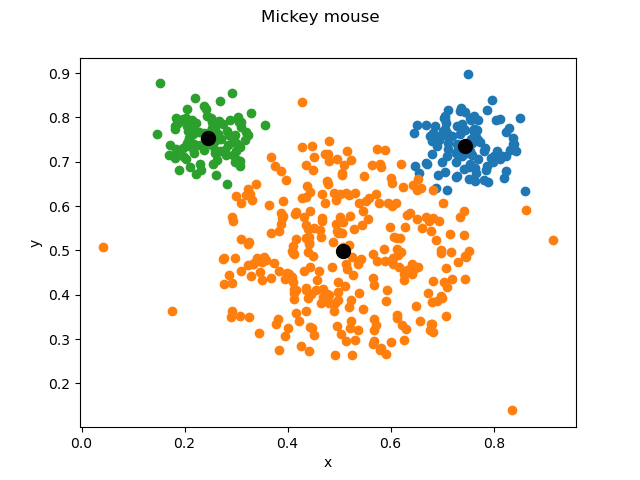
\includegraphics[width=\textwidth / 2]{plots/mickey_em3}
    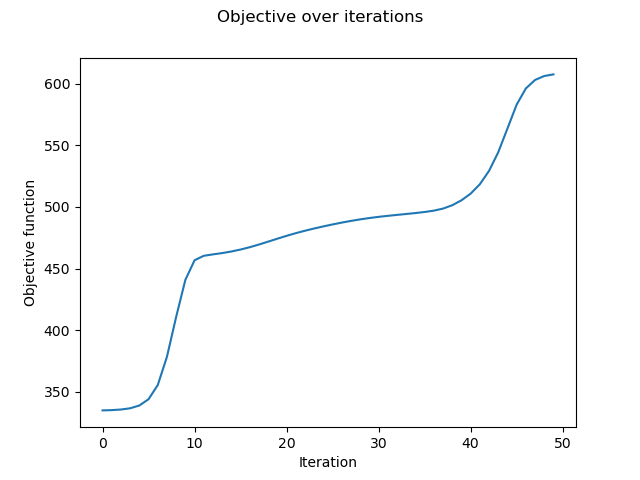
\includegraphics[width=\textwidth / 2]{plots/mickey_em3_likelihood}
    Compared to the original data (see \ref{subseq:kmeans}), the EM-algorithm provides a very good result.
    Nearly all of the points are correctly classified, although the algorithm still cannot identify the outliers as such.
    We also see none of the problems the K-means algorithm had, where parts of the big cluster were assigned to one of the smaller clusters.

    This is also reflected in the final values of $\pi$.
    We can see clearly that the bigger cluster got a bigger weight, while the two smaller clusters have a similar, smaller weight.\\
    Inital value of $\pi$: \texttt{Init pi: [0.33333333 0.33333333 0.33333333]}\\
    Final value of $\pi$: \texttt{Pi: [0.60036228 0.20177808 0.19785964]}

    \subsection{Summary and comparison of two algorithms}

    Which algorithm works better for the Mouse dataset? Why? Explain by comparing the plots of the original data, after K-means clustering, and after EM clustering using GMM.\\
    - As stated above, the EM algorithm has worked better for this dataset. There are more correctly classified points as with the K-means algorithm. K-means struggled with classifying some of the points that are close to the smaller clusters, EM didn't.\\

    Are there noisy data points (outliers) in  the original data? Is K-means robust to noise? Is EM robust to noise?\\
    - There are some outliers in the dataset. Assuming "robust to outliers" means the algorithms can identify and handle outliers, neither K-Means nor EM are robust to outliers. Both algorithms cannot identify which of the points are outliers.\\

    What is the main difference between kmeans and em algorithms? \\
    - K-means focuses on optimizing cluster centers and assigning data points to these centers based on distance. It assumes equal-sized spherical clusters. EM focuses on estimating parameters for a probabilistic model (like GMM) and assigning probabilities to data points for each cluster. K means is simpler and more efficient, EM is more flexible/ can handle more different types of data distributions. \\

    Which concrete distribution is given by initial values for pi (if yo check the code, there we have pi\_k = 1 / K)? Can you relate the final values of pi\_k with clusters (e.g., the maximum value in pi is for which cluster)? \\
    - The initial distribution assumes equal weights for all K clusters. The final values of pi\_k correspond to the weights assigned to each cluster after the algorithm is done. The maximum value in pi corresponds to the biggest, most dominant cluster. Smaller values in pi\_k will correspond to the two smaller clusters at the top of the bigger cluster.\\

    In the EM algorithm, the covariance matrices are updated in each iteration. K-means does not have this parameter. What shape of clusters does K-means tend to produce? Hence, what are the assumed (implicit) covariance matrices for clusters in K-means? \\
    - K-Means tends to produce spherical clusters. When calculating distances between data points and centroids, K-means considers each feature independently. The covariance matrix is a diagonal covariance with equal elements along the diagonal. The equal values along the diagonal indicate that there is no correlation between the features.\\

    \section{Image segmentation using K-means -- Code analysis}

    1.1) What does a single sample represent? \\
    - A single sample represents a pixel in the image i.e. a tuple of three values that represents a specific colour. \\

    1.2) What is this step (taking a subsample) equivalent to? \\
    In this step we are creating a training dataset from the data of the original image in order to train a model with it. This is a common approach in machine learning. With this training dataset the model can learn colour patterns in the image and group similar pixels together. \\

    1.3) Why is it important to take a random subsample of the original image (and not, for example, the first 1000 samples of the original image)? \\
    - The goal of this code is to reduce the number of colors needed to display the image. The subsample is supposed to be a diverse representative of the colours present in the whole image. In this image the first 1000 samples would most likely correspond to only a few different shades of blue since the upper left corner is only sky. To accurately represent the colours in the image, pixels/ samples from all over the image should be included in the training set.\\

    2) What does variable $n\_colors$ represent, i.e., which hyperparameter or parameter relevant for K-means? (State also if it is a hyperparameter or parameter.) \\
    - $n\_colors$ is a hyperparameter for the KMeans algorithm. It specifies the number of colors the image should be reduced down to (in this case from 96,615 unique colors to 64).\\

    3) What is the equivalent function (that we implemented ourselves) to fit method (see code line 56)? \\
    - The equivalent function to the fit method would be kmeans function we implemented in task 2. \\

    4) What is the equivalent function (that we implemented ourselves) to predict method? \\
    - The equivalent function to the predict method would be the $assign\_samples\_to\_clusters$ method. Like the predict method it assigns data points to clusters based on their proximity to the centroids.\\

    5) What does variable $codebook$ represent, i.e., which hyperparameter or parameter relevant for K-means? (State also if it is a hyperparameter or parameter.)
    - The $codebook$ variable represents a random selection of cluster centers. $codebook$ is not a parameter or hyperparameter for the KMeans algorithm. It is used as a comparison in the code to demonstrate the difference between the quantized image obtained using KMeans and a random codebook.

    
    
    


\end{document}

%%%%%%%%% end snippet
